\documentclass[11pt]{article}
\usepackage[margin=1in]{geometry}
\usepackage{iftex}
% arXiv builds with pdfLaTeX (CJKutf8); local previews with tectonic use XeTeX (xeCJK + a system font).
\ifXeTeX
  \usepackage{fontspec}
  \setmainfont{Times New Roman}
  \usepackage{xeCJK}
  \setCJKmainfont{Songti SC}
  \newcommand{\zh}[1]{#1}
\else
  \usepackage[T1]{fontenc}
  \usepackage{times}
  \usepackage{CJKutf8}
  \newcommand{\zh}[1]{\begin{CJK*}{UTF8}{gbsn}#1\end{CJK*}}
\fi
\usepackage[numbers,sort&compress]{natbib}
\usepackage{graphicx,booktabs,amsmath,amssymb,xcolor,microtype,multirow,enumitem}
\usepackage[hidelinks]{hyperref}
\setlist{itemsep=1pt,topsep=3pt}

\title{Shared Backbone, Separate Minds?\\What Qwen3 Speech Models Inherit from Their LLM}
\author{%
  Jiexiong Zhao\,(\zh{赵杰雄})\thanks{Correspondence: \texttt{anweat@outlook.com}.}\\
  Beijing Jiaotong University, Beijing, China
}
\date{}

\begin{document}
\maketitle

\begin{abstract}
Speech models are increasingly built on top of large language models, and it is often assumed that they ``inherit'' the LLM's knowledge. We test what is actually shared inside one model family, Qwen3, whose LLM, ASR and TTS models have identically shaped decoders. We combine four kinds of evidence: shrink-corrected weight lineage, layerwise representation similarity with random-network controls, causal stitching of LLM states into the TTS, and end-to-end measurement of what the TTS actually says. The ASR decoder shares the LLM backbone at every depth (CKA .91--.98), and its weight drift carries function: replacing it with equal-norm noise destroys transcription. The TTS shares only its first layers, and similarity does not imply substitutability: linearly mapped LLM states recover at most 0.30 of the text effect inside the TTS, while the same procedure between two unrelated TTS models recovers 0.93--0.97. We then ask whether a specific piece of LLM knowledge, the reading of Mandarin polyphones, can be handed to the TTS. Hidden states of the LLM encode the reading (probe minority recall .83 vs.\ .74 for the TTS text path), yet the LLM cannot say it when prompted (.46--.48 at 0.6B--4B). A small discrete interface, a pronunciation codebook written into the TTS input, fixes the spoken reading regardless of where the reading comes from; end to end it raises minority-reading accuracy from .41 to .80 with an LLM head and to .87 with a retrained supervised G2P, which beats the LLM. An on-device pipeline (int8 G2P, 114\,MB, 39\,ms per sentence, unmodified TTS) lifts minority readings from .52 to .85 under both an ASR detector and an independent three-judge panel. Inheritance is narrower than assumed: ASR reuses the LLM; TTS needs a narrow interface and a specialist front end, not the LLM. All criteria were fixed before the corresponding outputs existed; a multi-listener human study is in preparation.
\end{abstract}

\section{Introduction}

Recent speech systems reuse LLM decoders as their backbone: ASR models attach an audio encoder to an LLM, and many TTS models are LLMs fine-tuned to emit speech tokens \citep{qwenaudio,qwen2audio,cosyvoice2,sparktts,llasa}. This invites two claims that are rarely separated. A \emph{deployment} claim: if the backbone is shared, one copy could serve several functions on a device. A \emph{knowledge} claim: the speech model inherits what the LLM knows, so the LLM can be used to make speech better.

Both claims are testable at the level of weights, representations and behaviour, and they need not hold together. We study the Qwen3 family \citep{qwen3}, where the LLM, its ASR \citep{qwen3asr} and its TTS \citep{qwen3tts} decoders have identical shapes, so that weights and hidden states can be compared layer by layer without alignment tricks. We ask four questions:
\begin{enumerate}
  \item \textbf{Lineage.} Which models descend from which, once a common shrinkage term is removed from weight differences?
  \item \textbf{Representation.} At which depths do ASR and TTS compute what the LLM computes?
  \item \textbf{Causality.} Where representations are similar, can LLM states replace the speech model's own?
  \item \textbf{Knowledge transfer.} Can a concrete piece of LLM knowledge, the context-dependent reading of a Chinese character, reach the TTS, and through what interface?
\end{enumerate}

\paragraph{Contributions.}
(1) A shrink-corrected weight atlas showing that the Qwen3 family is a tree rather than a star around the base model, and that naive delta cosines create spurious kinship (\S\ref{sec:lineage}).
(2) Evidence that ASR shares the LLM backbone at all depths and that its drift carries function, but that a ``shared backbone plus low-bit residual'' deployment that looks free in simulation loses to independent 4-bit models on a real on-device kernel (\S\ref{sec:asr}).
(3) Evidence that TTS shares only shallow layers, and that similarity does not imply substitutability under causal stitching (\S\ref{sec:tts}).
(4) A ``readable but not speakable'' result for polyphone knowledge, and a pronunciation codebook: a narrow discrete interface that lets any reading source control a TTS without phoneme input, evaluated by synthesizing audio and judging it with independent ASR models (\S\ref{sec:pron}).
Several results are negative, and we report them as such.

All decision criteria (thresholds, comparison sets, primary judges) were written into the experiment scripts before the outputs they judge were produced; analyses added after seeing results are labelled exploratory. Code and per-item outputs are released.\footnote{\url{https://github.com/anweat/qwen3-inheritance}}

\section{Related work}
\label{sec:related}
\paragraph{Model differences, merging and shared deployment.} Task vectors \citep{ilharco2023task} and model merging \citep{yadav2023ties,yu2024dare} treat a fine-tuned model as a base plus a difference, and delta compression stores that difference in very few bits so that many fine-tunes can share one base \citep{liu2024bitdelta}. These methods assume that the difference is small and structured. We test that assumption across functions rather than across tasks of one function. We also show that a shared shrinkage of weights toward zero inflates cosines between differences and creates spurious kinship, so it must be removed before lineage is read from weights. On the deployment side, low-bit quantization of LLM weights is well studied \citep{dettmers2022int8}; our ASR results add that a shared-base scheme which matches a 4-bit baseline in simulation can lose to the runtime's own 4-bit quantizer and kernels.

\paragraph{Comparing representations, and similarity versus function.} Linear CKA \citep{kornblith2019cka} and SVCCA \citep{raghu2017svcca} are the standard tools for comparing layers across networks, and CKA's reliability has been questioned \citep{davari2023cka}. Model stitching \citep{lenc2015equivariance,bansal2021stitching} asks the causal question instead: can one network use another's states? Closest to our framing, \citet{hsu2026geometric} show for speech LLMs that geometric alignment between speech and text representations does not imply that the model uses them in the same way. We find the same gap for speech \emph{output}: shallow TTS layers resemble the LLM, yet linearly mapped LLM states cannot replace them. Massive activations and attention sinks \citep{sun2024massive,xiao2024sinks} are present in Qwen3; in our cross-family check they also break linear CKA between nearly identical models, which is why we report that check only as supporting evidence.

\paragraph{Probing: encoding versus saying.} Probes with control tasks \citep{hewitt2019control} separate what a representation makes linearly available from what a probe learns by itself, and work on latent knowledge \citep{burns2023latent} shows that models can encode answers they do not state. Our polyphone results fit this pattern. The reading is linearly decodable from LLM states, but much of the probe's accuracy is already available from neighbouring token embeddings, and the model does not produce the reading when asked.

\paragraph{Inside speech LLMs.} Recent analyses of audio-language models such as Qwen2-Audio and SALMONN compare speech and text representations layer by layer \citep{xiang2025modalitygap}, decode adapter outputs into the LLM's text vocabulary \citep{ogunremi2025transcribe}, or explain why text ability degrades after speech adaptation \citep{wang2025textdegradation}. These works study models that take speech as \emph{input} to an LLM. We instead compare dedicated ASR and TTS decoders with the LLM they came from, at the level of weights, representations and causal substitution, including a model that produces speech.

\paragraph{LLM-based TTS and its evaluation.} Codec language models \citep{valle} cast TTS as next-token prediction over speech tokens, and several recent systems start this language model from a pretrained LLM: CosyVoice~2, Spark-TTS and Llasa \citep{cosyvoice2,sparktts,llasa}. Qwen3-TTS \citep{qwen3tts} follows the same talker design; an independent study characterises its conditioning interfaces and failure modes, including with a listening test \citep{baroudi2026qwen3tts}. TTS intelligibility is usually measured by transcribing the audio with an ASR model. We go further, checking whether a specific reading was spoken: we validate several recognizers \citep{sensevoice,paraformer,whisper} as pronunciation judges against human speech, and restrict them to the contrasts on which they pass.

\paragraph{Mandarin polyphone disambiguation.} Polyphone disambiguation is a classic front-end task for Mandarin TTS. g2pM introduced the CPP benchmark \citep{g2pm}, and g2pW conditions a BERT classifier on candidate readings \citep{g2pw}. These systems output pinyin, which a phoneme-input TTS can consume directly. Character-input TTS models such as the Qwen3 talker cannot take pinyin. Our pronunciation codebook is a way to connect any such G2P to them without retraining the TTS.

\section{Setup}
\label{sec:setup}

\paragraph{Models.} Qwen3 at 0.6B: Base, Instruct, Guard-Gen, Guard-Stream, Embedding, Reranker, ASR, Forced\-Aligner, TTS-Base and TTS-Custom\-Voice (all with 28-layer, 1024-wide decoders); at 1.7B: Base, ASR, TTS and VL models. For ASR we use the text decoder of the thinker; for TTS the talker decoder. Cross-family checks use Llasa-1B, Spark-TTS-0.5B and the LM of CosyVoice~2 (\S\ref{sec:tts}).

\paragraph{Data.} A fixed text corpus of 75 segments of 128 tokens (Chinese and English documents, code and spoken-style text) for representation analyses; 800 held-out utterances from AISHELL-1, FLEURS and five Chinese dialect sets for ASR \citep{aishell1,fleurs}; and for pronunciation, the CPP test set \citep{g2pm} split into a hard set of minority readings (230 items, 77 characters) and majority readings (90 items), plus two natural-text sets: 76 positions in real-speech transcripts (21 characters) and 131 positions drawn from CPP test sentences in their natural distribution (``natural2'', 46 characters). Only characters that are a single token and readings without tone sandhi or neutral tone are included.

\paragraph{Judging what the TTS says.} For an item with gold reading $g$ and competitor $a$, we synthesize the sentence (O) and two references in which the character is replaced by single-reading homophones of $g$ and of $a$ ($R_g$, $R_a$). The \emph{detector} is an ASR model (Qwen3-ASR) teacher-forced on the left context; it scores the log odds of $g$ over $a$ for the next token, centred at the midpoint of the two references. Because the detector shares the Qwen family, we also validate a \emph{panel} of three non-Qwen recognizers, SenseVoice, Paraformer and Whisper large-v3-turbo \citep{sensevoice,paraformer,whisper}, voting by strict majority. On known-reading clips and 89 hand-labelled real-speech positions, each panel judge passed the preset bar (.90) for contrasts that differ in initial or final (real speech .90--.94), but no judge reached it for tone-only contrasts on real speech (best .889), and none can reliably report a third reading (Table~\ref{tab:judges}). We therefore use the panel only on segmental contrasts.

\paragraph{Statistics.} Differences are paired by item; 95\% intervals come from a bootstrap that resamples characters (groups), not items, with 4{,}000 resamples. Where we state a verdict, the criterion was fixed in advance.

\section{Weight lineage}
\label{sec:lineage}

A common way to read lineage is the cosine between weight differences $W_a-B$ and $W_b-B$ relative to a base $B$. This is misleading when fine-tuning shrinks weights: every difference then contains a component along $-B$, and unrelated models look related. We instead remove the best scalar multiple of the base, $R=W-\alpha B$ with $\alpha=\langle W,B\rangle/\langle B,B\rangle$ per matrix, and compare residuals. With the shrink term included, TTS and ASR differences have cosine .46; after removing it, 0.00.

Figure~\ref{fig:lineage} shows the 0.6B family. Distances form a tree: models in one branch are within .005--.16 of each other, different functions are at least .25 apart, and the TTS models are about 1.5 from everything. Residual cosines identify branches: Guard-Stream and Reranker descend from Instruct (.99, .96), Guard-Gen and Embedding from Base (residual cosine to Instruct $\approx$0), ForcedAligner from ASR (.39). TTS-0.6B has residual cosine 0.000 with every text model and appears to be trained from scratch; TTS-1.7B starts from its Base but is almost entirely rewritten. A complementary measure, the conditional entropy of 4-bit codes given a reference, says the same: Guard-Gen costs 0.12 bit per weight given Base (96.6\% saving), ASR-0.6B 2.25 bits given Instruct (37\%), and TTS 3.6 bits, i.e.\ nothing is saved.

Weight distance is not functional distance. ASR is three times farther from Base than Instruct is (.34 vs.\ .12), yet on text its next-token distribution is closer to Base (Jensen--Shannon .06--.10 vs.\ .14--.18).

\begin{figure}[t]
  \centering
  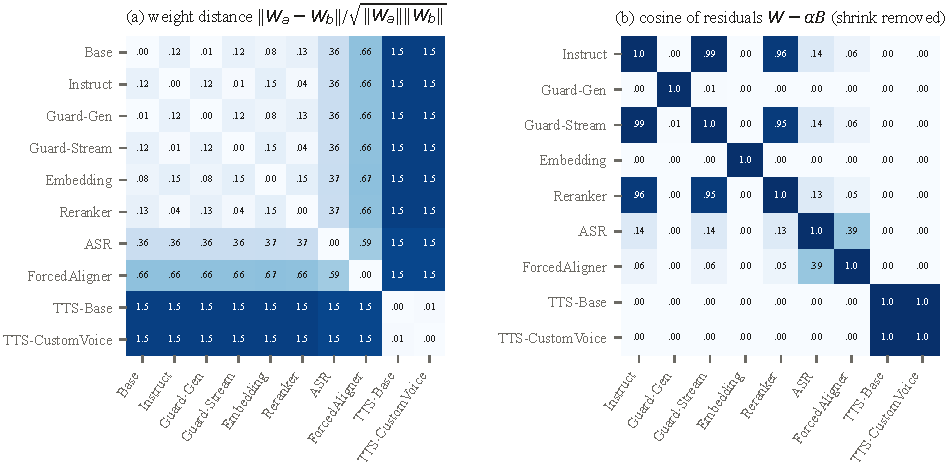
\includegraphics[width=\linewidth]{figures/fig_lineage.pdf}
  \caption{Weight lineage of the Qwen3-0.6B family. (a) Pairwise relative distance of decoder weights. (b) Cosine between residuals after removing the shrink toward the base, which separates branches that raw delta cosines conflate.}
  \label{fig:lineage}
\end{figure}

\section{ASR inherits the backbone}
\label{sec:asr}

\paragraph{Representations.} On the fixed corpus, the ASR decoder's text-position states have debiased linear CKA .91--.98 with Base at the same depth across all 28 layers (Figure~\ref{fig:cka}a), above Instruct at several depths; a randomly initialized network gives .11--.20 and token shuffling gives 0.00. Attention agrees as well: matched heads have Jensen--Shannon divergence .04--.06, against .35--.48 for random pairings.

\paragraph{Drift carries function.} The ASR decoder can be written as the Base weights plus a residual. Quantizing the base to 4 bits and the residual to 2 bits (per-block, four levels) leaves transcription intact in simulation (LibriSpeech WER .075 vs.\ .077 for the full model under the same 64-token cap). Replacing the residual by noise of equal norm, or by the base itself, gives 100\% error. Scaling the residual by $t$ is lossless for $t\geq .85$ and fails at $t=.7$. A per-layer analysis shows that any single layer except the first and last can be reverted at little cost, but damage accumulates: reverting eight layers fails completely. A 1\% set of ``transcription'' neurons per layer stops transcription when zeroed while leaving text modelling untouched, and a matched set of ``text'' neurons does the reverse (double dissociation; Appendix~\ref{app:asr}).

\paragraph{But sharing does not pay on a real device.} On 800 real utterances (15 sets), simulated 2-bit residuals matched independent symmetric 4-bit quantization. We then re-ran the comparison with packed weights and real kernels (Apple M4, MLX \citep{mlx}), with criteria fixed in advance (Table~\ref{tab:runtime}). Against the runtime's native affine 4-bit quantizer, the shared base plus residual was worse by +1.31 [+0.74, +1.88] points of error and 34\% slower end to end; counting per-group scales, the residual costs 2.5--3.0 bits rather than 2, and LLM plus ASR saves only about 110\,MB of decoder weights. The simulated equivalence came from a weak 4-bit baseline (relative error .099 vs.\ .082 for the runtime's quantizer). Accuracy on Chinese and dialects was unchanged (+0.06 [$-$0.58, +0.63]); the loss lies in other languages.

\begin{table}[t]
  \centering\small
  \caption{Qwen3-ASR-0.6B decoder on a real on-device kernel (M4, MLX), 800 utterances, language given. Bytes are ASR-specific decoder weights including scales.}
  \label{tab:runtime}
  \begin{tabular}{lccccc}
    \toprule
    Scheme & Error & Zh + dialect & Other & End to end (median) & Bytes \\
    \midrule
    bf16 & 9.93\% & 9.10 & 10.69 & 693 ms & 881 MB \\
    Independent Q4, group 32 & 11.36\% & 9.14 & 13.39 & 526 ms & 275 MB \\
    Shared Q4 + 2-bit residual, group 32 & 12.68\% & 9.20 & 15.85 & 707 ms & 165 MB \\
    Independent Q4, group 64 & 11.69\% & 8.98 & 14.16 & 508 ms & 248 MB \\
    Shared Q4 + 2-bit residual, group 64 & 13.31\% & 9.07 & 17.17 & 704 ms & 138 MB \\
    \bottomrule
  \end{tabular}
\end{table}

\section{TTS inherits only shallow layers}
\label{sec:tts}

\begin{figure}[t]
  \centering
  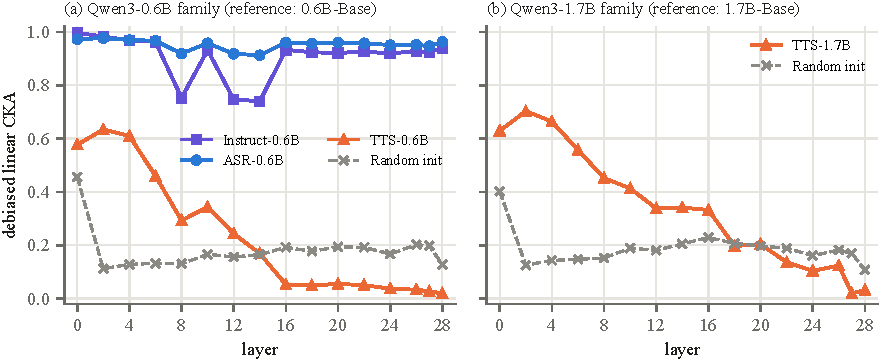
\includegraphics[width=\linewidth]{figures/fig_cka.pdf}
  \caption{Layerwise debiased linear CKA between text-position states of each model and the same-size Base on identical text (4{,}800 tokens). ASR tracks Base at all depths; both TTS models, whether trained from scratch (0.6B) or from Base (1.7B), share only shallow layers and fall to or below the random-network control in deep layers. The dips of Instruct at layers 8, 12, 14 coincide with heavy-tailed activations.}
  \label{fig:cka}
\end{figure}

\paragraph{Shallow similarity.} With the TTS in non-streaming mode, text tokens pass through the talker like ordinary self-attention inputs, so the same text positions can be compared. TTS-0.6B reaches CKA .58--.63 with Base in layers 0--4 and falls below the random control from layer 16 on; TTS-1.7B, which starts from Base, behaves the same way, from .70 at layer 2 to .12 at layer 26 (Figure~\ref{fig:cka}). Linear prediction is asymmetric: Base states predict TTS states better than the reverse (layer 12: $R^2$ .28 vs.\ .14).

\paragraph{The talker reads text in a narrow window.} Masking which layers of the audio rows may attend to text shows that TTS-0.6B reads text almost only at layer 6 (keeping only that read: cross-entropy 1.480 vs.\ 1.466 unmasked, 2.48 without text) and TTS-1.7B from layer 3. The talker is effectively ``text encoder, single read-out, audio decoder''.

\paragraph{Similarity is not substitutability.} We overwrite the text positions at layer $k$ with ridge-mapped states and block earlier reads, so text can reach the audio only through the supplied states. The target is teacher-forced first-codebook cross-entropy on 100 held-out real utterances; ``recovered'' is $(\mathrm{CE}_\text{no text}-\mathrm{CE})/(\mathrm{CE}_\text{no text}-\mathrm{CE}_\text{native})$. LLM states recover at most 0.30 (1.7B, $k=1$) and about zero beyond (Figure~\ref{fig:stitch}). This is not a failure of the method: the same ridge maps between two TTS models whose weights are unrelated recover 0.93--0.97, and native text corrupted to the LLM map's $R^2$ still recovers $\geq$.92. In five of six settings, the LLM's token embedding alone does better than its contextual state, so what little transfers is token identity, not context processing. Taking deeper LLM layers (4--27) does not help.

\begin{figure}[t]
  \centering
  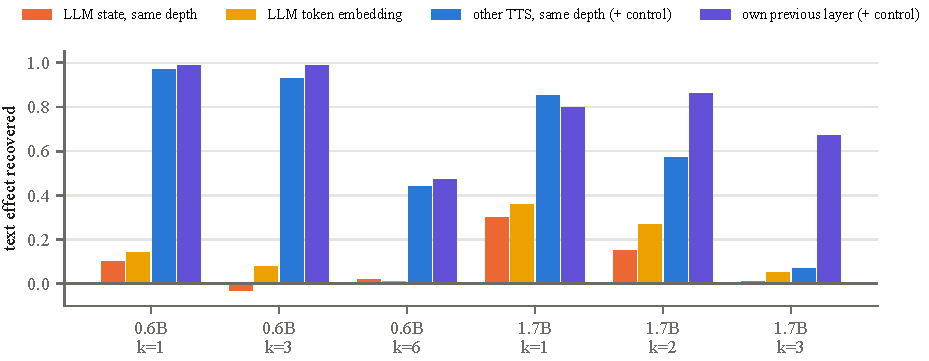
\includegraphics[width=\linewidth]{figures/fig_stitch.pdf}
  \caption{Causal stitching into the TTS talker at layer $k$. Fraction of the native text effect on first-codebook cross-entropy recovered by each linearly mapped source (1 = native text, 0 = no text).}
  \label{fig:stitch}
\end{figure}

\paragraph{Other families (supporting evidence only).} We repeated the lineage and CKA analysis on three LLM-initialized TTS models from other families. Weights confirm the lineage (Table~\ref{tab:families}): Llasa-1B descends from Llama-3.2-1B \citep{llama3}, Spark-TTS from Qwen2.5-0.5B \citep{qwen25}, and the LM of CosyVoice~2 from Qwen2-0.5B-Instruct \citep{qwen2}, whose weights are identical to the ``CosyVoice-BlankEN'' checkpoint shipped with it; all were heavily changed (residual cosine .20--.66 vs.\ .99 for Instruct vs.\ Base). Their CKA profiles have the same shape as Qwen3's, from .37--.56 in the first third of layers to about .2, near the random control, in the last third. However, linear CKA across these models was dominated by massive activations \citep{sun2024massive}: Qwen2.5 without a BOS token turns the first text token into an attention sink. After removing outlier tokens and dimensions, our preset positive control (Instruct vs.\ Base $\geq$.9 at every layer) still failed (Qwen2.5 layer 24: .86; Llama layer 15: .67), so by our own rule this measurement does not support a cross-family verdict.

\begin{table}[t]
  \centering\small
  \caption{Lineage of LLM-initialized TTS from other families (shrink-corrected residual cosine to the closest LLM) and CKA to that LLM (first / last third of layers, outlier-filtered). The CKA rows did not pass our positive control and are descriptive only. CosyVoice~2's CKA was computed against Qwen2.5-0.5B, before its true base was identified.}
  \label{tab:families}
  \begin{tabular}{llcccc}
    \toprule
    TTS & Base found by weights & Cosine & CKA first & CKA last & Random first \\
    \midrule
    Llasa-1B & Llama-3.2-1B & .66 & .56 & .20 & .16 \\
    Spark-TTS-0.5B & Qwen2.5-0.5B & .20 & .37 & .19 & .11 \\
    CosyVoice~2 LM & Qwen2-0.5B-Instruct & .31 & (.41) & (.23) & (.11) \\
    \midrule
    \multicolumn{2}{l}{Reference: Instruct vs.\ Base (Qwen2.5, Llama-3.2)} & .99 & -- & -- & -- \\
    \bottomrule
  \end{tabular}
\end{table}

\section{What can be handed to the TTS: pronunciation}
\label{sec:pron}

If the TTS does not reuse the LLM's context processing, can it still receive a specific piece of the LLM's knowledge? We use Mandarin polyphones as a pilot: the reading of characters such as \zh{行} (\emph{x\'ing}/\emph{h\'ang}) depends on context, and the TTS takes characters, not phonemes.

\paragraph{The TTS often says the wrong reading.} On the hard set, TTS-0.6B says the minority reading only .515 [.396, .629] of the time (1.7B: .470), against .72--.77 for majority readings. On natural text the problem is smaller (.794 on natural2; .921 on real-speech transcripts).

\paragraph{The LLM encodes the reading.} Ridge probes on hidden states, trained per character with at most 100 examples, recover minority readings better from the LLM (.83 at 0.6B and 1.7B) than from the TTS text path (.74--.75; difference +8.2 [+5.1, +11.7] points). Much of this is lexical: concatenated embeddings of five neighbouring tokens already give .77, and the LLM's contextual gain over them is +6.2 [+2.6, +10.1] points. A separate probe on single-reading characters refutes the idea that LLM embeddings ignore pronunciation: they predict initial, final and tone of held-out characters 23--55 points above a random network, though less well than TTS embeddings.

\paragraph{But it cannot say it.} Prompted zero-shot to choose the reading, Qwen3-0.6B, 1.7B and 4B score .46--.48 on minority readings, below the TTS's own audio (.522) and far below the probes, with no gain from scale (Figure~\ref{fig:pron}a). With thinking enabled (exploratory), 4B reaches .517; its reasoning often identifies the word and meaning correctly and then states the wrong reading.

\paragraph{A pronunciation codebook.} To let any reading source control the TTS, we write a reading vector into a rare token and substitute it for the character, leaving generation unchanged. The vector for reading $r$ is the mean text embedding of all single-reading, single-token characters with reading $r$ (rescaled to the members' mean norm, excluding the reference homophones). This alone controls the spoken reading with balanced accuracy .977 [.953, .996] (0.6B) and .982 (1.7B), on par with substituting a homophone. The codebook has 1{,}334 entries ($\approx$5\,MB at 16 bit) and covers 407 of the 650 CPP readings.

\paragraph{The LLM adds little; a specialist G2P adds more.} Feeding the reading predicted by a head into the codebook and synthesizing audio, minority-reading accuracy rises from .410 to .795 with a head on the TTS's own layer 6, .795--.808 with an LLM layer-8 head, and .872 with g2pW \citep{g2pw} retrained on CPP with its official recipe (test accuracy .990, matching the published .991) (Figure~\ref{fig:pron}b). On the same items, g2pW beats the LLM head by +.126 [+.073, +.186], and their errors barely complement each other (oracle union .922). The LLM's own contribution over the TTS's head is +.057 [+.004, +.112] at layer 8, a weak result given that five layers were compared without correction. The off-the-shelf g2pW release, trained on a different standard, loses to both heads, which would have suggested the opposite conclusion.

\begin{figure}[t]
  \centering
  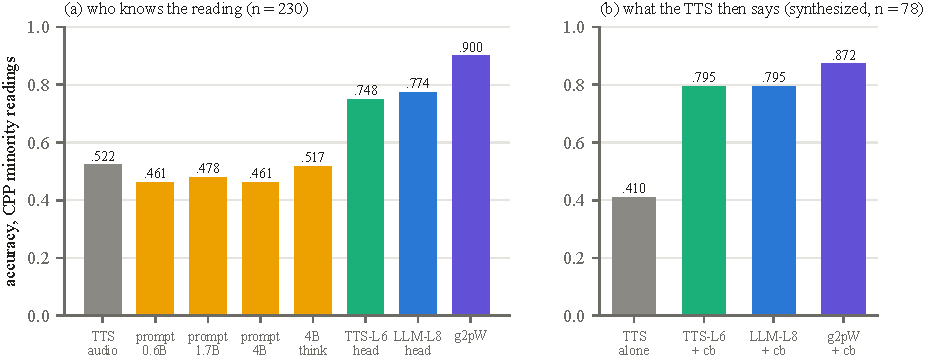
\includegraphics[width=\linewidth]{figures/fig_pron.pdf}
  \caption{CPP minority readings. (a) Accuracy of the reading chosen by each source: what the TTS actually says, the LLM prompted zero-shot, linear heads on TTS layer 6 and LLM layer 8, and a retrained g2pW. (b) Accuracy of the synthesized audio when that reading is written into the TTS through the pronunciation codebook (cb), judged by the ASR detector on the 78 items with codebook coverage.}
  \label{fig:pron}
\end{figure}

\paragraph{An on-device pipeline.} We assemble text $\rightarrow$ g2pW (int8, 114\,MB, 39\,ms per sentence on an M4 CPU; agreement with fp32 .998) $\rightarrow$ codebook $\rightarrow$ unmodified Qwen3-TTS-0.6B, rewriting every eligible polyphone in the sentence, plus a user dictionary that overrides the G2P. Under the detector (primary, preset), minority readings rise from .522 to .848 (+.326 [+.209, +.447]) and natural2 from .794 to .916 (+.122 [+.034, +.221]), meeting both preset criteria (useful: lower bound $>0$; safe: lower bound $>-.05$). The three-judge panel agrees on the hard set (+.344 [+.192, +.497]) but sees only a non-significant gain on natural2 (+.059 [$-$.060, +.206]) (Figure~\ref{fig:pipeline}). On real-speech transcripts most targets sit inside multi-character tokens and are left alone (28\% rewritten; +.013). A 21-sentence dictionary demonstration of names and places goes from .286 (TTS) and .524 (G2P only) to 21/21.

\begin{figure}[t]
  \centering
  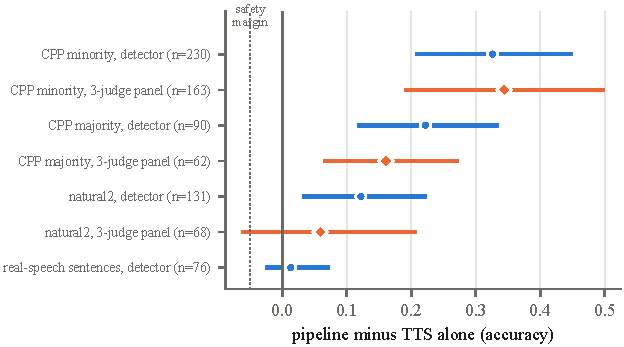
\includegraphics[width=.62\linewidth]{figures/fig_pipeline.pdf}
  \caption{On-device pipeline minus TTS alone, paired by item, with character-bootstrap 95\% intervals. The panel is restricted to segmental contrasts. Dotted line: preset safety margin ($-.05$).}
  \label{fig:pipeline}
\end{figure}

\paragraph{Where the risk is (exploratory).} Rewritten targets are almost always right afterwards (panel, natural2: .80 $\rightarrow$ .98). The risk is in characters left alone next to rewritten ones. In a fresh-sample follow-up on 86 such sentences, the preset test was inconclusive ($-$.125 [$-$.266, +.011]), but the loss concentrated where an edit sat within two characters of the target ($-$.232 vs.\ 0 farther away), e.g.\ rewriting \zh{禺} in \zh{番禺} made the TTS fall back to the default reading of \zh{番}. A word-level rule (segment with jieba \citep{jieba}; do not rewrite inside a word that contains an un-rewritable polyphone) improved 7 and worsened 0 of 22 affected sentences, but these came from only two characters, so its preset criterion (lower bound $>0$) was not met (+.227 [.000, +.360]).

\section{Discussion and lessons}
\label{sec:discussion}

\paragraph{What is inherited.} Within one family, ASR genuinely reuses the LLM: representations match at all depths and the residual on top of the LLM is small and functional. TTS reuses only the bottom of the stack, and its deep text processing is its own; the shape repeats in three other families, though our cross-family measurement did not pass its control. For knowledge, the useful path is not to feed LLM states into the TTS or to ask the LLM in words, but to read a discrete decision out of hidden states with supervision and pass it through a narrow interface. On polyphones, a supervised G2P trained on the same data is better still, so the interface, not the LLM, is the transferable contribution.

\paragraph{Methodological lessons.}
\begin{enumerate}
  \item Remove shrinkage before reading lineage from weight differences; otherwise unrelated models appear related.
  \item A compression scheme that matches a baseline in simulation must be re-checked against the runtime's own quantizer and kernels; here the baseline, not the scheme, changed.
  \item Linear CKA across models needs outlier handling and a same-family positive control; massive activations can produce near-zero similarity between nearly identical models.
  \item ASR judges of pronunciation are reliable for segmental contrasts only; tones and third readings need human listeners.
\end{enumerate}

\section{Limitations}
\begin{itemize}
  \item \textbf{No multi-listener human evaluation yet.} All TTS correctness numbers come from ASR-based judges. A pilot with one listener on 36 original sentences agreed with the detector on all 30 answered items but marked 6 as neither reading. A blind study with at least three listeners, catch trials and preset hypotheses has been prepared and will be reported in a revision.
  \item \textbf{One family for causal claims.} Stitching and the ASR analyses were run on Qwen3 only; the cross-family check is descriptive.
  \item \textbf{Gold labels.} CPP gold readings were checked against a dictionary by a single annotator (an AI assistant); some apparent G2P errors look like label errors. A second annotator is pending.
  \item \textbf{Scope of the pilot task.} Polyphones are one task; prosody, named entities or cross-sentence reference might favour the LLM. Only single-token characters were tested; neutral tone and sandhi were excluded.
  \item \textbf{Multiple comparisons.} We fixed primary criteria per experiment but did not correct across experiments; layer-wise comparisons in \S\ref{sec:pron} are flagged where they matter.
\end{itemize}

\section{Conclusion}
In the Qwen3 family, the ASR decoder is the LLM with a small, functional residual, while the TTS shares only its first layers and cannot use the LLM's states. The LLM's knowledge of how to read a character is present but not speakable; it reaches the TTS only through a narrow discrete interface, and a specialist G2P serves that interface better than the LLM. Inheritance is narrower than the shared architecture suggests.

\section*{Acknowledgements}
This work would not have been possible without openly released models, data and software. We thank the Qwen team at Alibaba for the Qwen3 family studied here---the base and instruct LLMs, Qwen3-ASR, Qwen3-TTS, the forced aligner and the guard models---and for publishing technical reports detailed enough to make layer-by-layer comparison possible. We thank the authors of Llasa, Spark-TTS and CosyVoice~2 for open weights and code from other families, which made the cross-family check possible, and the Llama, Qwen2 and Qwen2.5 teams for the base models those systems build on. The recognizers used as pronunciation judges come from the FunAudioLLM project (SenseVoice) and Paraformer, both released through FunASR, and from Whisper (OpenAI). The polyphone baselines and benchmarks are due to the g2pM and g2pW authors, including the CPP test set. We are grateful to the providers of the speech data used in the ASR and judging analyses, AISHELL-1 and FLEURS, and to the open-source tools that made the on-device measurements reproducible, in particular MLX and jieba.

The experiments, analyses and this manuscript were prepared with substantial assistance from Claude (Anthropic), under the author's direction; every number reported here was produced by scripts in the released repository and checked against their outputs, and all remaining errors are the author's.

\bibliographystyle{plainnat}
\bibliography{refs}

\appendix
\section{Additional ASR results}
\label{app:asr}

\begin{table}[h]
  \centering\small
  \caption{Zeroing 1\% of neurons per layer (26 layers) in ASR-0.6B: a double dissociation between transcription-specific and text-specific neurons.}
  \begin{tabular}{lcccc}
    \toprule
    Zeroed neurons & Prefix agreement & Transcript CE & Transcript & Text CE (code) \\
    \midrule
    Random & 1.000 & 0.034 & normal & 2.343 \\
    Text-specific & 1.000 & 0.030 & normal & \textbf{2.915} \\
    Transcription-specific & \textbf{0.128} & \textbf{0.566} & stops at once & 2.338 \\
    \bottomrule
  \end{tabular}
\end{table}

The first token receives a massive activation at layer 2 (about $+6{,}800$ on one dimension, written by the same five MLP neurons in Base, Instruct and ASR) and acts as an attention sink: attention to it rises from 3\% at layer 2 to 71\% at layer 26. Removing the spike doubles text cross-entropy; a 64-token attention window that keeps the first token is nearly lossless (2.24 vs.\ 2.19 on code), whereas dropping it is not (3.53).

\section{Judge validation}
\label{app:judges}

\begin{table}[h]
  \centering\small
  \caption{Candidate pronunciation judges. ``Bal.'' = balanced accuracy on TTS clips of known reading; ``Real'' = accuracy on hand-labelled real-speech positions. Preset bar: .90 on both.}
  \label{tab:judges}
  \begin{tabular}{lcccc}
    \toprule
    & \multicolumn{2}{c}{Initial/final differ} & \multicolumn{2}{c}{Tone only} \\
    Judge & Bal.\ (TTS) & Real & Bal.\ (TTS) & Real \\
    \midrule
    Charsiu (centred) & .971 & .659 & .980 & .804 \\
    SenseVoice & .996 & \textbf{.935} & .971 & .804 \\
    Paraformer & .992 & \textbf{.903} & .979 & .889 \\
    Whisper large-v3-turbo & .985 & \textbf{.917} & .960 & .826 \\
    Qwen3-ASR (detector, not in panel) & .996 & .935 & .957 & .733 \\
    \bottomrule
  \end{tabular}
\end{table}

\section{Pronunciation codebook and pipeline details}
\label{app:pipeline}
The codebook entry for a reading is the mean input embedding of its single-reading, single-token member characters, rescaled to the members' mean norm; readings with fewer than three members get no entry. A position is rewritten automatically only if the character is a CPP polyphone, g2pW returns a toned reading, the reading is not neutral tone and the character is not \zh{一} or \zh{不}, the reading has a codebook entry, and the character is a token of its own. Dictionary entries override g2pW and are applied even inside multi-character tokens.

\end{document}
